%
% ground_segment.tex
%
% Copyright (C) 2021 by SpaceLab.
%
% GOLDS-UFSC Documentation
%
% This work is licensed under the Creative Commons Attribution-ShareAlike 4.0
% International License. To view a copy of this license,
% visit http://creativecommons.org/licenses/by-sa/4.0/.
%

%
% \brief Ground segment chapter.
%
% \author Gabriel Mariano Marcelino <gabriel.mm8@gmail.com>
%
% \institution Universidade Federal de Santa Catarina (UFSC)
%
% \version 0.1.0
%
% \date 2020/06/06
%

\chapter{Ground Segment} \label{ch:ground-segment}

\section{Hardware}

\subsection{Antennas}

There are two antennas in the ground station: One for VHF and one for the UHF band. The main characteristics of these antennas can be seen in \autoref{tab:grs-antennas}

\begin{table}[ht]
    \centering
    \begin{tabular}{lccc}
        \toprule[1.5pt]
        \textbf{Characteristic} & \textbf{VHF Antenna}  & \textbf{UHF Antenna}  & \textbf{Unit} \\
        \midrule
        Brand                   & M$^{2}$               & Cushcraft             & - \\
        Model                   & 2MCP14                & A719B                 & - \\
        Type                    & Yagi                  & Yagi                  & - \\
        Number of elements      & 14                    & 19                    & - \\
        Frequency range         & 143-148               & 430-450               & MHz \\
        Gain                    & 12,34                 & 15,5                  & dBi \\
        Power rating            & 1500                  & 2000                  & W \\
        Boom length             & 3,2                   & 4,1                   & m \\
        Longest element         & 1,02                  & 0,34                  & m \\
        Weight                  & 2,72                  & 2,55                  & kg \\
        \bottomrule[1.5pt]
    \end{tabular}
    \caption{Main characteristics of the ground segment antennas.}
    \label{tab:grs-antennas}
\end{table}

More information about the VHF and UHF antennas can be found in \cite{2mcp14} and \cite{a719b} respectively.

\subsection{Rotor}

.

\subsection{Amplifiers}

\subsubsection{Power Amplifier}

PA\nomenclature{\textbf{PA}}{\textit{Power Amplifier}}...

\subsubsection{Low Noise Amplifiers}

LNA\nomenclature{\textbf{LNA}}{\textit{Low Noise Amplifier}}...

\subsection{Radios}

.

\subsection{Processing and Control}

.

\section{Satellite Tracking}

To track the satellite and for orbit prediction, the GPredict software \cite{gpredict} will be used. Gpredict is a real-time satellite tracking and orbit prediction application. It can track a large number of satellites and display their position and other data in lists, tables, maps, and polar plots (radar view). Gpredict can also predict the time of future passes for a satellite, and provide you with detailed information about each pass. Gpredict is free software licensed under the GNU General Public License. A picture of the main window of GPredict can be seen in \autoref{fig:gpredict}.

\begin{figure}[!ht]
    \begin{center}
        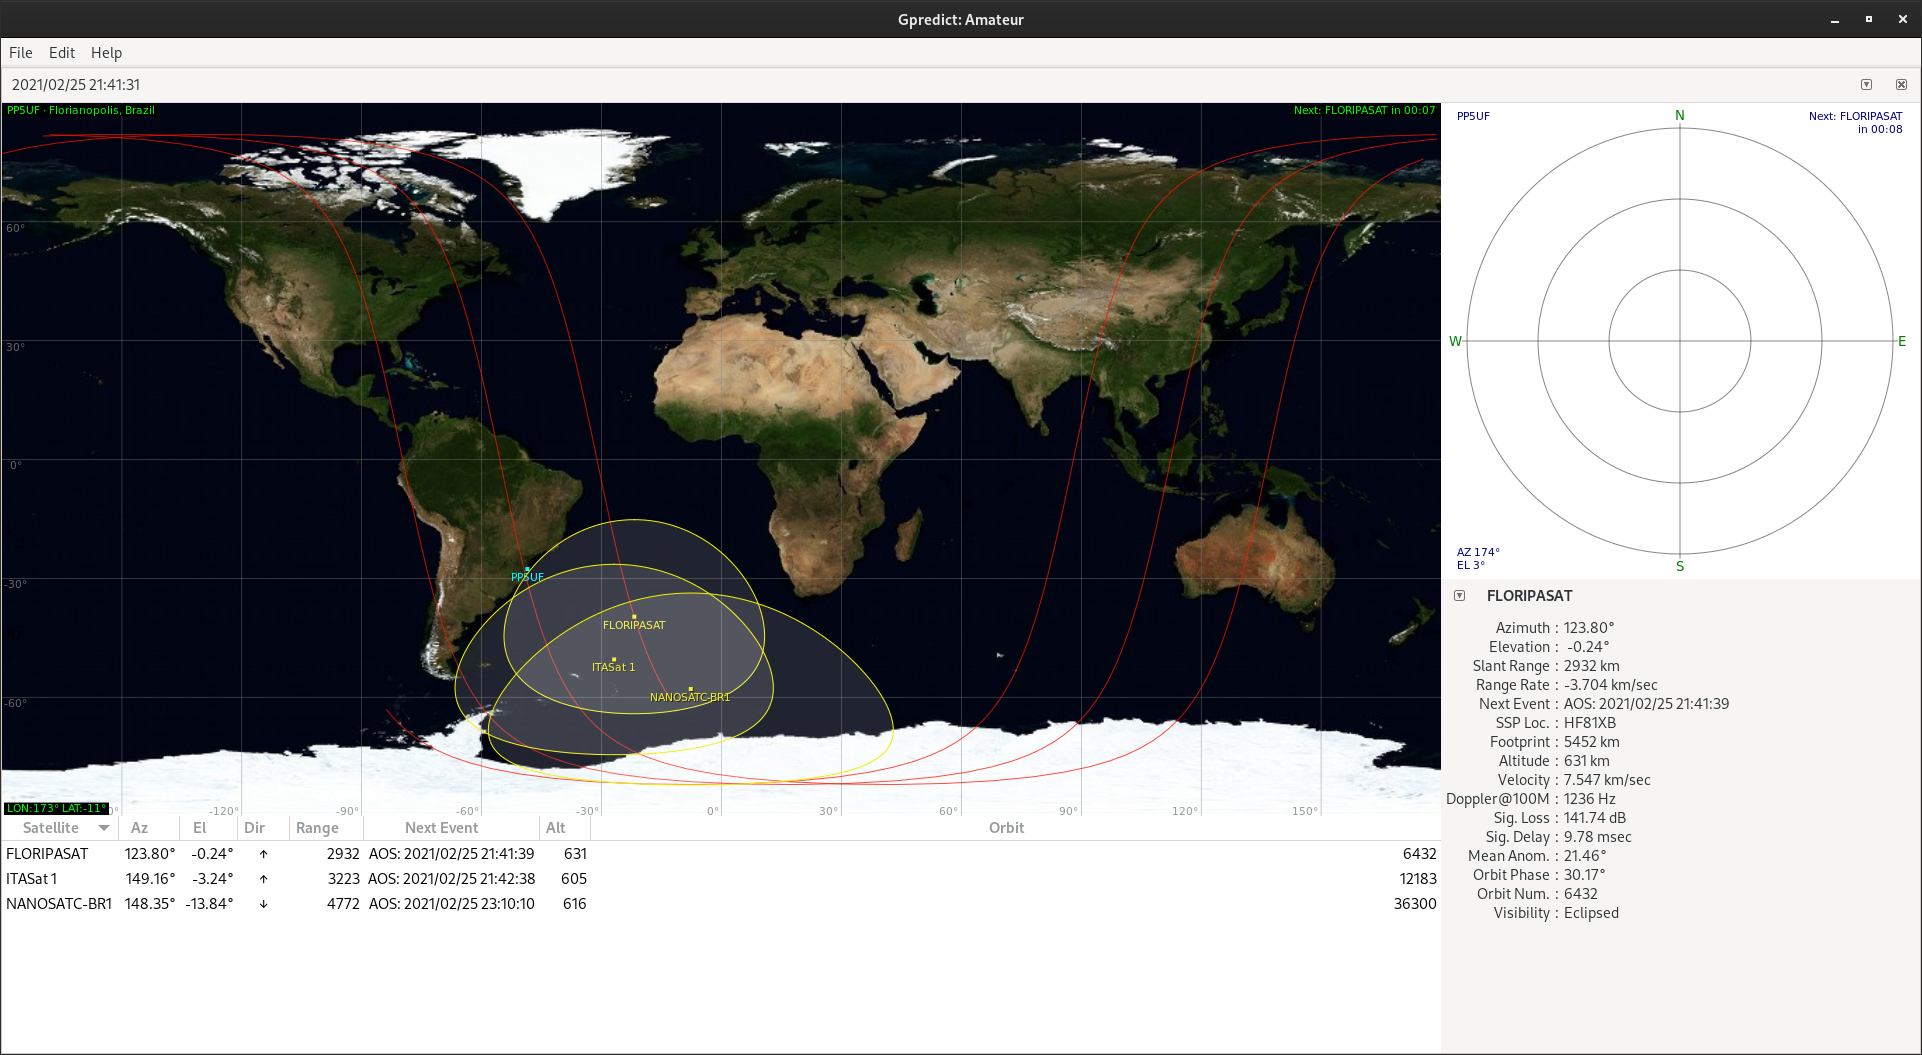
\includegraphics[width=\textwidth]{figures/gpredict.png}
        \caption{Main window of GPredict.}
        \label{fig:gpredict}
    \end{center}
\end{figure}

\section{Packet Decoding}

\cite{spacelab-decoder}

\begin{figure}[!ht]
    \begin{center}
        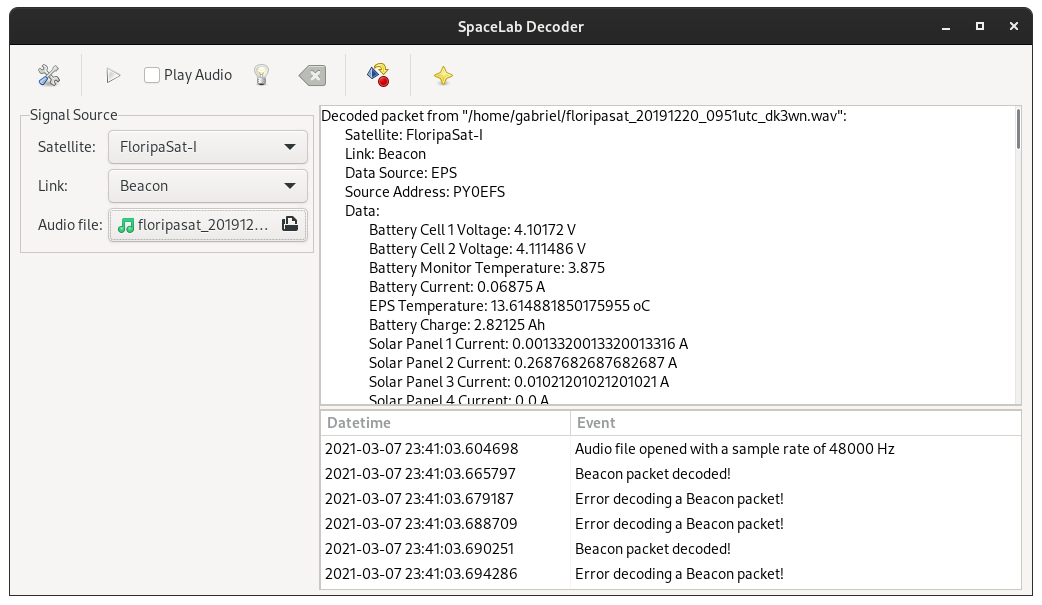
\includegraphics[width=\textwidth]{figures/spacelab-decoder.png}
        \caption{Main window of the SpaceLab Decoder application.}
        \label{fig:spacelab-decoder}
    \end{center}
\end{figure}

\section{PCDs}

PCD\nomenclature{\textbf{PCD}}{\textit{``Plataforma de Coleta de Dados'', or Data Collection Platform}}...
